\section{Cosmology}
\subsection{Questions}
\begin{enumerate}
\item Put on a timeline, and describe the principal events in the thermal history of the
universe, from $kT = 10$ TeV to $kT = 0.1$ eV.
\item Give a semi-quantitative discussion of the connection between flucuations of the
cosmic microwave background on angular scales of arcminutes to degrees, and the
baryonic structures (galaxies, clusters, correlations of galaxies) observed in the local
universe, redshift $z < 0.5$.
\item Which elements/isotopes are produced in Big Bang Nucleosynthesis and in what
quantities? Explain qualitatively how the yield of each depends on the cosmic baryon
density and why.
\end{enumerate}

\subsection{Measuring Distances}
The basic concept of distance is the distance ladder, which is basically 
different techniques used to measure distances farther and farther away.  
There is overlap between the different techniques, which allows the next 
technique to be calibrated by the previous one.  The only problem with this 
is errors and uncertainties at the bottom of the ladder propogate all the 
way up.  

The first step is parallaxes, which are reliable out to $\sim100$ pc or so.  As 
the Earth moves around the Sun, the apparent positions of stars will change 
slightly relative to more distant fixed background stars.  The distance 
to an object in parsecs is defined to be $\frac{1}{p}$ where $p$ is the 
parallax in arcseconds.  One useful trick to know for quickly converting 
between angular size and physical size- the physical size in AU of something 
$d$ parsecs away with an angular size of $\theta$ arcsec is just $\theta d$.  
So, for example, if a star and planet are $1$ pc away and are separated by 
$1$ arcsec, the planet is $1$ AU from the star.  Parallax is the only 
distance indicator that is not model dependent or reliant on some other 
calibration.  

Out to distances of $\sim1$ kpc, main sequence fitting can be used to find 
distances to main sequence stars.  If the spectral type of a star is measured, 
and the absolute magnitude of that spectral type is known from a closer 
star with a parallax distance, the difference between apparent and absolute 
magnitude gives the distance to the new star.  

This has been done for clusters of stars that contain Cepheid variables, 
leading to the next step in the distance ladder.  Cepheids are horizontal 
branch high mass stars in the instability strip of the HR diagram (see Stars 
notes).  Cepheids are useflu as distance indicators because their periods 
are tightly correlated with their luminosities by 
\begin{equation}
\log{\frac{L}{L_{\odot}}}\sim2.4+1.2\log{\frac{P}{days}}
\end{equation}
So by measuring the period of pulsation, the intrinsic luminosity can be 
determined, giving a distance.  Nearby galaxies (within $20$ Mpc) are close 
enough that individual Cepheids can be observed and used to get distances.  

Advantages:  Bright ($M_V\sim-4$ to $-7$), so the can be used in other galaxies.  
Also, we understand the physics behind their pulsation well, and can identify 
them based on their period.  

Disadvantages:  Cepheids are relatively rare since they correspond to short 
phases of stellar evolution and high masses.  Also, there are uncertainites 
about systematics of the period-luminosity relation like how it depends on 
metallicity and color.  

The tip of the red giant branch method is applicable out to similar distances 
as Cepheids.  Stars at the top of the red giant branch, right before He flash, 
have a known absolute magnitude of $-4$.  This point also corresponds to a 
drop-off in the frequency of stars, so once this is found and its brightness 
is measured, the distance can be determined.  

Advantages: Stars are bright and method is relatively precise and 
well-understood.  

Disadvantages:  Only works for old populations.  

Another method is planetary nebulae luminosity functions.  Planetary nebulae 
have an observed cut-off in luminosity at absolute magnitude $-4.5$.  The 
physics behind the cut-off is understood, and planetary nebulae can be found 
in all types of galaxies.  

For galaxies out to $\sim100$ Mpc, there are several methods to get distances, 
including the Tully-Fisher relation, globular cluster  
luminosity functions, and surface brightness fluctuations.  The Tully-Fisher 
relation is an observed correlation between the rotational velocity of 
spiral galaxies and their luminosity:
\begin{equation}
L\propto v_{rot}^4
\end{equation}
The rotational velocity is usually measured by HI $21$ cm line width.  The 
problems with this method are the relation has $\sim10-20$\% scatter, and 
the physics behind it are not well understood.  The fundamental plane gives 
similar relations for elliptical galaxies.  Globular clusters have well-defined empirical luminosity functions that can be used as 
standard candels.  Globular clusters have a peak at an absolute magnitude 
of $-6.6$.  An advantage of this method is it is not affected by dust.  
However, deep photometry is needed to measure the luminosity function, and 
this method is not as precise as others.  Surface brightness fluctuations 
involve measuring the surface brightness (flux per solid angle) in several 
regions of the same galaxy.  The observed surface brightness depends on the 
number of stars in the region, which should be similar in the different 
patches.  If the average number of stars is N, the Poisson scatter in the 
number of stars (and thus the brightness) will be $\frac{1}{\sqrt{N}}$.  
The number of stars per solid angle will also depend on distance as 
$N\propto r^2$.  So the observed scatter $\sigma\propto\frac{1}{r}$.  This 
relation can be calibrated using nearby galaxies.   

For even more distant galaxies (out to $\sim1$ Gpc), Type Ia supernovae 
can be used as standard candles to get a distance.  A tight correlation 
exists between the shape of a Ia lightcurve and the luminosity of the 
supernova, so by measuring the shape of the light curve, the distance can 
be determined.  This method is very precise, but we still don't understand 
the mechanism for a type Ia supernova.  Type Ia supernovae can be observed 
into the Hubble flow, so a plot of distance versus redshift can be used 
to determine the cosmological parameters.  The main problem with all these 
methods so far is they rely on calibrations from other methods.  One of the 
main goals of the Hubble Space Telescope was to improve these calibrations 
and determine $H_0$ more precisely.  The main focus was to better calibrate 
Cepheids and the distance to the LMC and SMC, which other methods are based 
on.  The HST $H_0$ Key Project determined $H_0=72\pm3\pm7$ km/s/Mpc.

Two methods that don't need calibration, but instead are model dependent 
are the S-Z effect (see section in Radiative) and gravitational lense 
time delays.  If a background quasar is lensed, variability in the quasar 
will be seen at different times on different sides of the lense, since the 
path length is different.  If the mass distribution of the lense is known, 
then the ratio of the path length difference to the source distance and lense 
distance can be determined.  Since the time delay is known, the path length 
difference can be calculated, giving the distance to the lense and the 
background quasar.  The modeling is very complicated however.  

\subsection{Age of the Universe}
An estimate of the age of the Universe is the Hubble time 
$t_H=1/H_0=4.4\times10^{17}h_{70}^{-1}$ s.  The exact age depends on the other 
cosmological parameters.  Other methods to get a lower limit on the age include 
globular cluster ages, white dwarf cooling times, and nucleocosmochronology 
(that's a mouthful).  Globular clusters are some of the oldest objects 
we can observe, so their ages give good lower limit to the age of the 
Universe.  The observed main sequence turnoff of a globular cluster can be 
combined with stellar isochrones to determine an age.  Uncertainties in 
the isochrone models and the distances to the clusters complicate this, 
but this methods gives lower limits ranging from around $10$ to $15$ Gyr.  
White dwarfs can also be used to age date globular clusters.  Higher 
mass stars turn into white dwarfs after only a few tens of Myr, so the 
white dwarfs will be $\sim$the same age as the cluster.  White dwarfs cool 
as they age in a fairly well understood way, so the luminosity of the 
dimmest white dwarfs in a cluster gives the age of the cluster.  There are 
still uncertainties in the cooling models though, and these white dwarfs are 
extremely faint, so this has only been done for one cluster, but the age 
agrees with the main sequence turnoff age.  Measuring abundance ratios of 
radioactive elements with Gyr or 10 Gyr half lives can also provide an estimate 
of the age.  This is difficult because the lines of these elements tend to be 
very weak in stars, but the measurements made so far give ages in the range of 
about $10-15$ Gyr.  All these methods are in agreement with the age determined 
from cosmological parameters.  

\subsection{Expansion of the Universe Tests}
Tolman Test:\newline
Observe something with a uniform surface brightness at different redshifts.  
Surface brightness is just flux per unit solid angle, so 
\begin{equation}
B=\frac{f}{d\Omega}
\end{equation}
\begin{equation}
B=\frac{L}{D_L^2}\frac{D_A^2}{dl^2}
\end{equation}
In a Euclidean, non-expanding Universe, $D_L=D_A$, so surface brightness should 
be constant for objects of constant $L/dl^2$.  In an expanding Universe, 
$D_L=D_A(1+z)^2$, so $B\propto(1+z)^{-4}$.  The intercept of the surface 
brightness scaling relations for elliptical galaxies make a good standard 
surface brightness.  Observations of clusters at different redshifts match 
$B\propto(1+z)^{-4}$.  

Hubble Diagrams:\newline
Hubble diagrams use standard candels or standard rulers to plot luminosity 
distance or angular diameter distance vs. redshift.  The shape of the 
curve gives information about the cosmological parameters.  For example, 
if the Universe has a lower density or positive $\Lambda$, it will have 
expanded faster and be larger today.  We know the Hubble constant today, 
so to slow down to this expansion rate would require more time, so the 
Universe would be older.  Since the Universe is larger, at a given 
redshift, objects would be further away, so they would look fainter and 
smaller.  A higher density Universe would behave the opposite way.  Plots 
of luminosity/angular diameter distance (or some proxy like magnitude or 
angular size) vs. redshift would show this (see Figure \ref{fig:hubble}).

\begin{figure}[!h]
\begin{center}
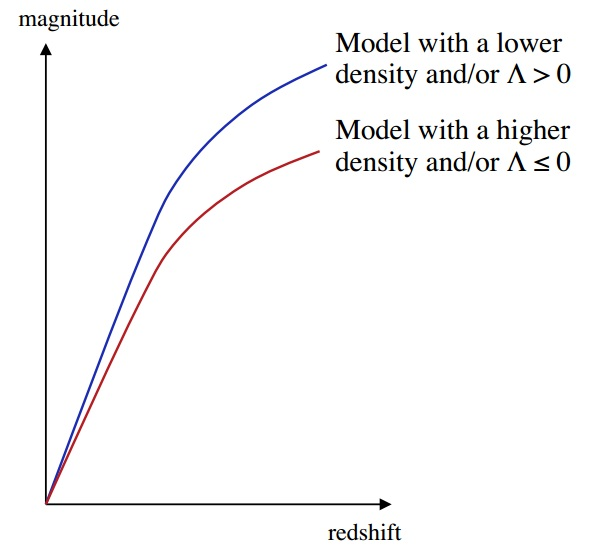
\includegraphics[width=\textwidth]{hubble.jpg}
\end{center}
\caption{A Hubble Diagram for different cosmological parameters.
\label{fig:hubble}}
\end{figure}

Early attempts at this used galaxies, clusters, and radio sources as standard 
candles and standard rulers, but galaxy and cluster evolution effects 
dominated over the effects of different cosmologies.  The use of type Ia 
supernovae (standard candles) and CMB fluctuations (standard rulers) provided 
much better tests.  

In these tests, biases from missed sources must be taken into account, as well 
as the K correction.  The idea behind the K correction is if we measure the 
light from a galaxy in a certain bandpass in our frame, the light we are seeing 
is from a bluer region of the spectrum, and this region is narrower by a 
factor of (1+z).  The bandpass emitted by the galaxy is redshifted and 
stretched when it reaches us.  This effect depends on redshift, so it must be 
taken into account when looking at galaxies at different redshifts.  The 
ratio of the flux in our frame to the flux in the galaxy's frame as a function 
of redshift has been computed for different types of galaxies and for different 
bandpasses.  

Using type Ia supernovae or CMB fluctuations indivually creates a degeneracy 
between $\Omega_{\Lambda}$ and $\Omega_M$ (here, $\Omega_M$ is density of 
baryonic and dark matter).  Combining these tests, however, breaks the 
degeneracy, and results in $\Omega_{\Lambda}\sim0.7$ and $\Omega_M\sim0.3$.

Another cosmological test is galaxy and cluster counts.  Plotting 
source counts vs magnitude (as a proxy for redshift) gives information 
on the density of the Universe.  A Universe with lower denstiy or higher 
$\Lambda$ will be larger, therefore there will be more sources to observe, 
so the curve will be higher.  A Universe with higher density will be smaller, 
and have a lower curve.  Galaxy evolution makes things difficult.  Galaxies 
were brighter in the past, so there will be extra counts at brighter 
magnitudes.  Also, because galaxies merge, there were more faint pieces in 
the past, which produces extra counts at fainter magnitudes.  To avoid this, 
really need redshifts of these galaxies.  Cluster counts rely on the 
assumption that we know what the number density of distant clusters should 
be based on the number density of nearby ones.  In a low density, older 
Universe, clusters could have formed further back in time, so we'd expect 
to see lots of distant ones.  In a higher density, younger Universe, clusters 
would only just be forming now, so we wouldn't see many distant ones.  

The combination of all these tests helps to better constrain the cosmological 
parameters and break degeneracies.  The results (I think these are pre-Planck) 
are shown in Table \ref{tab:cosmo}.

\begin{table}[H]
\centering
\begin{tabular}{c c}
\hline\hline
Parameter&Value\\
\hline
$t_0$ & $13.82\pm0.05$ Gyr\\
$H_0$ & $69$ km/s/Mpc\\
$\Omega_{baryon}$ & $0.04$\\
$\Omega_{matter}$ & $0.31$\\
$\Omega_{\Lambda}$ & $0.69$\\
\hline
\end{tabular}
\caption{Cosmological Parameters \label{tab:cosmo}}
\end{table}

\subsection{Contents of the Universe}
Baryonic Dark Matter:\newline
Observations show that the Universe's luminous matter density is only 
$\Omega_{lum}\sim0.005$, compared to $\Omega_{baryon}\sim0.04$.  This comes 
from measuring the amount of light we see, and combining this with a mass to 
light ratio.  So there is a lot of missing baryonic matter.  Two possibilities 
are massive compact halo objects (MACHOs) and cold H$_2$ gas clouds.  The most 
likely explanation looks to be warm/hot gas in galaxies groups that never 
collapsed into galaxies.  This gas would have temperatures of $\sim10^5-10^6$ 
K.  The emission from this gas would be in the far-UV/soft x-rays, which would 
be absorbed by the ISM and not be detectable.  There have been some potential 
detections through UV absorption though.  

Non-baryonic Dark Matter:\newline
This is the actual dark matter we usually talk about.  Galaxies and x-ray 
gas in clusters have typical velocity dispersions of $500-1500$ km/s, with 
cluster radii of $3-5$ Mpc.  Using the virial theorem, this gives masses 
of $10^{14}-10^{15}\ M_{\odot}$.  The total luminosity of clusters is only 
$\sim10^{12}\ L_{\odot}$, so the mass to light ratio of these clusters 
is in the hundreds.  This means lots of dark matter.  In individual galaxies, 
flat rotation curves (spirals) and flat velocity dispersions (ellipticals) 
cannot be accounted for with just the visible matter, implying the presence of 
dark matter.  The density profile of a spiral galaxy can be found by 
balancing rotation with gravity.  
\begin{equation}
\frac{v^2(r)}{r}=\frac{GM(r)}{r^2}
\end{equation}
If density is constant, then
\begin{equation}
M(r)=\frac{4}{3}\pi r^3\rho
\end{equation}
and
\begin{equation}
v(r)=r\sqrt{\frac{4\pi G\rho}{3}}
\end{equation}
This velocity profile is seen in the bulges of spirals (see Figure 
\ref{fig:vcurve}).  If the density is assumed to follow a power law
\begin{equation}
\rho(r)=\rho_0\left(\frac{r}{r_0}\right)^{-\alpha}
\end{equation}
then
\begin{equation}
v(r)=\sqrt{\frac{4\pi G\rho_0r_0^{\alpha}}{3-\alpha}}r^{1-\alpha/2}
\end{equation}
For $v(r)$ to be constant, need $\alpha=2$.  So $\rho\propto r^{-2}$ and 
$M(r)\propto r$.  This is called a singular isothermal sphere.

\begin{figure}[!h]
\begin{center}
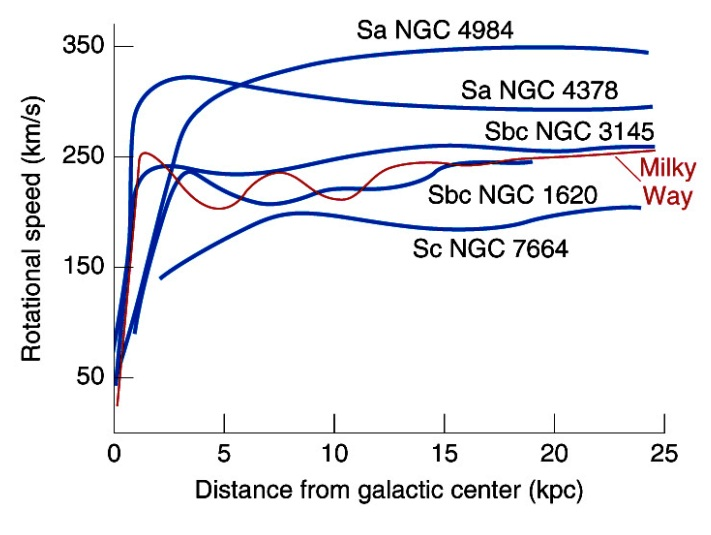
\includegraphics[width=\textwidth]{vcurve.jpg}
\end{center}
\caption{Velocity curves of spiral galaxies. \label{fig:vcurve}}
\end{figure}

Small irregular galaxies can have mass to light ratios of $100$, 
meaning they are even more dark matter dominated than big galaxies.  This is 
thought to be because the shallow gravitational potential of these galaxies 
allows the baryonic matter to be expelled, leaving only the dark matter.  

Candidates for dark matter include massive neutrinos (which we know exist, we 
just don't know how much exists), and theoretical particles like weakly 
interacting massive particles (WIMPS, not to be confused with the glorious 
society) and axions.  Modified Newtonian gravity is another, less popular 
possibility.  In terms of structure formation, dark matter is broken down into 
two classes- hot (HDM) and cold (CDM).  Hot dark matter would be relativistic 
particles such as neutrinos.  The relativistic speeds of HDM would smooth-out 
small-scale density fluctuations in the early Universe, so large structures 
would form first, and smaller structures would form later through fragmentation 
(top-down structure formation).  CDM would consist of slower moving 
particles like WIMPs or axions.  Small density fluctuations would not be 
affected, so small structures would form before large structures (bottom-up 
structure formation).  Most dark matter is probably CDM.  

Dark energy is a complete mystery.  We know the Universe's expansion is 
accelarating due to a cosmological constant $\Lambda$, with 
$\Omega_{\Lambda}\sim0.7$ (see expansion test section).  We don't know what 
dark energy actually is though.  


